%%%%%%%%%%%%%%%%%%%%%%%%%%%%%%%%%%%%%%%%%%%%%%%%%%%%%%%
%% Engineer & Master Thesis, LaTeX Template          %%
%% Copyleft by Piotr Woźniak & Artur M. Brodzki      %%
%% Faculty of Electronics and Information Technology %%
%% Warsaw University of Technology, Warsaw, 2019     %%
%%%%%%%%%%%%%%%%%%%%%%%%%%%%%%%%%%%%%%%%%%%%%%%%%%%%%%%

\documentclass[
    left=2.5cm,         % Sadly, generic margin parameter
    right=2.5cm,        % doesnt't work, as it is
    top=2.5cm,          % superseded by more specific
    bottom=3cm,         % left...bottom parameters.
    bindingoffset=6mm,  % Optional binding offset.
    nohyphenation=true % You may turn off hyphenation, if don't like. =false
]{eiti/eiti-thesis} % bazuje na clasie mwart

\nocite{*}

\usepackage[
    backend=bibtex,
]{biblatex}
\usepackage{csquotes}
\usepackage{hyperref}
\usepackage{algpseudocode}
\usepackage{algorithm}

\langpol % Dla języka angielskiego mamy \langeng
\graphicspath{{img/}}             % Katalog z obrazkami.
\addbibresource{bibliografia.bib} % Plik .bib z bibliografią

\makeatletter
\xpatchcmd\lst@MakeCaption{\protect\numberline{\thelstlisting}\lst@@caption}{\protect\numberline{\thelstlisting.}\lst@@caption}{}{}
%\makeatother
%\makeatletter
%\xpatchcmd{\LT@c@ption}{\protect\numberline{\thetable}}{\protect\numberline.{. \thetable . }}{}{}
\makeatother

\begin{document}

%--------------------------------------
% Strona tytułowa
%--------------------------------------
\RaportThesis
\instytut{Cyberbezpieczeństwa}
\kierunek{Telekomunikacja}
\specjalnosc{Techniki Teleinformatyczne}
\title{
    Akceleracja sprzętowa kryptoanalizy algorytmów kryptograficznych
}
\engtitle{ % Tytuł po angielsku do angielskiego streszczenia
    Hardware acceleration of cryptoanalysis of cryptograhpic algorithms
}
\author{Andrzej Tłomak}
\album{311450}
\promotor{dr. hab. inż. Mariusz Rawski}
\date{\the\year}
\maketitle

%--------------------------------------
% Streszczenie po polsku
%--------------------------------------
\streszczenie
Cel pracy
\slowakluczowe Krzywe eliptyczne, Kryptografia, Kryptoanaliza, CUDA, Algorytm~rho~Pollard'a

\newpage

%--------------------------------------
% Streszczenie po angielsku
%--------------------------------------
\abstract
The objective of this phase included a review of the literature describing the current State-of-Art \
in cryptoanalysis of systems \
based on Elliptic curves in Finite Fields. It involved getting deeper knowledge of theory
and mathematical fundation of Elliptic curves as well as setting up an environment
to develop implementation utillizing CUDA technology.
\keywords Elliptic curves, Cryptography, Cryptoanalysis, CUDA, FPGA, rho~Pollard~algorithm
\newpage

%--------------------------------------
% Oświadczenie o autorstwie
%--------------------------------------
\makeauthorship
\blankpage

%--------------------------------------
% Spis treści
%--------------------------------------
%\thispagestyle{empty}
\tableofcontents
%\blankpage

%--------------------------------------
% Rozdziały
%--------------------------------------
\newpage
\section{Wprowadzenie}

Wraz z rosnącą potrzebą zapewnienia poufności i integralności danych w systemach
informatycznych, kryptografia stała się jednym z filarów współczesnych rozwiązań
bezpieczeństwa. Kryptografia oparta na krzywych eliptycznych \textbf{ECC} ( \textit{Elliptic Curve Cryptography}) jest
obecnie jednym z najważniejszych standardów w tej dziedzinie, oferując wysoki
poziom bezpieczeństwa przy znacznie mniejszych rozmiarach kluczy w porównaniu
do tradycyjnych algorytmów, takich jak RSA \cite[]{Ao2016,Barker2016}.
Z tego powodu ECC znajduje szerokie zastosowanie w systemach o ograniczonych zasobach,
urządzeniach IoT ( \textit{Internet of Things}) czy urządzeniach mobilnych \cite[]{Thakur2022,Hammi2020}.

Bezpieczeństwo ECC opiera się na trudności rozwiązania problemu logarytmu
dyskretnego na krzywych eliptycznych. Jest to problem matematyczny, który w
praktyce nie ma efektywnego rozwiązania w rozsądnym czasie przy użyciu
współczesnych metod obliczeniowych. Do tej pory nie opracowano algorytmu
zdolnego rozwiązać ten problem w czasie podwykładniczym na komputerach klasycznych, dlatego
kryptoanaliza ECC wymaga dużych zasobów obliczeniowych \cite{Menezes2001}.
Z tego powodu, często wykorzystywane w tej roli są układy GPU \cite[]{Boss2015,Panetta2017,Bernstein2012},
FPGA \cite[]{Wenger2014,Mane2011,FPGA2008,Majkowski2008}
czy nawet konsole dla graczy \cite{Bos2010}.

Gwałtowny rozwój kart graficznych \textbf{GPU} ( \textit{Graphic Processing Unit})
oraz technologii \textbf{CUDA} ( \textit{Compute Unified Device Architecture}) znacznie zwiększył możliwości
przeprowadzania takich analiz. Choć rozwój ten był w dużej mierze napędzany
zapotrzebowaniem związanym z uczeniem maszynowym, jego zastosowanie w
innych dziedzinach, takich jak kryptoanaliza jest równie istotny.

Karty graficzne, dzięki architekturze zoptymalizowanej do równoległych obliczeń,
stały się narzędziem o kluczowym znaczeniu w dziedzinach wymagających intensywnego
przetwarzania danych. Platforma CUDA, opracowana przez firmę NVIDIA, umożliwia
wykorzystanie mocy obliczeniowej GPU do realizacji zadań takich jak
implementacja algorytmów kryptograficznych oraz analiza ich odporności na ataki.
CUDA pozwala na masywnie równoległe przetwarzanie danych, co ma kluczowe znaczenie
w implementacji algorytmu Rho Pollard'a, który w wersji równoległej, pozwala na efektywne
wykorzystanie możliwości GPU.

Chociaż GPU nie oferują wydajności i efektywności energetycznej 
porównywalnej z dedykowanymi układami, takimi jak FPGA czy ASIC, ich dostępność 
i stosunkowo niski koszt czyni je atrakcyjnym wyborem do obliczeń kryptograficznych. 
W obliczu rosnącej mocy obliczeniowej GPU oraz ich szerokiej dostępności, ciągła 
analiza odporności algorytmów kryptograficznych na ataki staje się jeszcze 
ważniejszym elementem ich rozwoju.

\subsection{Cel pracy}
Celem tej pracy jest realizacja systemu korzystającego z koprocesora GPU,
w celu przyśpieszenia obliczeń przy
rozwiązywaniu problemu logarytmu dyskretnego.
Implementacja została zoptymalizowana i dostosowana do obliczenia logarytmu
dyskretnego na krzywej eliptycznej ECCp-79, zaproponowanej w wyzwaniu \textit{The Certicom ECC Challenge} \cite{certicom-challange}.
\par
Głównymi elementami stworzonego systemu
jest program klienta wykonującego część algorytmu Rho Pollard'a na karcie graficznej Nvidia
z wykorzystaniem technologii CUDA i języka programowania CUDA C++,
oraz program serwera działający na CPU, odpowiedzialny za zarządzanie klientami i zbieranie wyników.
 Wyniki implementacji zostały porównane z innymi pracami
których celem była kryptoanaliza ECC z wykorzystaniem akceleracji sprzętowej.
\newpage % Zaleca się otwieranie rozdziału od nowej strony.
\section{Wstęp teoretyczny}


\subsection{Procesor graficzny}
DO UZUPEŁNIENIA
GŁÓWNIE SŁOWNICTWO oraz architektura SIMD
SM - streaming multiprocesor
BLOCK - grupa wątków, najbardziej granularny sposób rozpoczynania obliczeń
wątek - pojedyncza logiczna jednostka obliczeniowa, wykonuje instrukcje w grupach po 32
(rozgałęzienia powodują sekwencyjność w tej grupie 32) 
good practice: brak rozgałęzień w kodzie, jedna instrukcja, wiele danych

Hierarchia pamięci

\subsection{Krzywe eliptyczne}
Zakładając, że ciało $\mathbb{K}$ ma charakterystykę różną od 2 i 3,
oraz że stałe $a, b \in \mathbb{K}$ spełniają warunek:
\[4a^3 + 27b^2 \neq 0\]
nieosobliwą krzywą eliptyczną nad ciałem $\mathbb{K}$ definiuje się jako zbiór punktów $(x,y) \in \mathbb{K} \times \mathbb{K}$,
spełniających równanie:
\[y^2 = x^3 + ax + b\]
wraz ze specjalnym punktem w nieskończoności $\mathcal{O}$, który pełni rolę elementu neutralnego
w działaniach grupowych
\cite{Stinson2021}.
\begin{figure}[H]
    \centering 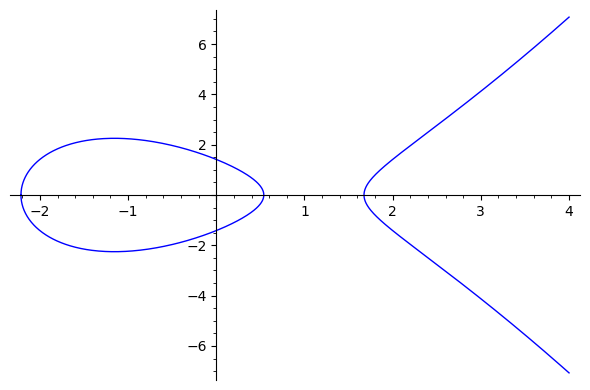
\includegraphics[width=0.8\linewidth]{sage/krzywa_-4_2.png}
    \caption{Krzywa eliptyczna $y^2=x^3-4+2$ nad ciałem liczb rzeczywistych}
\end{figure}

Krzywe eliptyczne zdefiniowane na liczbach rzeczywistych nie są kluczowe w
systemach kryptograficznych \cite*{Stinson2021}, ale takie ustawienia
pozwalają na prostsze przedstawienie niektórych zagadnień
np. dodawnie punktów na krzywej.


\subsubsection{Dodawanie punktów na krzywej eliptycznej}
Odpowiednie zdefiniowanie operacji dodawania punktów na krzywej eliptycznej
pozwala otrzymać grupę abelowa, złożoną z punktów krzywej oraz punktu w nieskończoności jako
elementu neutralnego.
\newline
\indent
Geometrycznie, dodawanie punktów na krzywej eliptycznej nad ciałem liczb rzeczywistych można przedstawić
jako połączenie dwóch punktów $P$ i $Q$ prostopadłą linią, która przecina krzywą w trzecim
punkcie, $R'$. Następnie, wynikowy punkt $R$, będący sumą $P+QP+Q$, znajdujemy przez
odbicie punktu $R'$ względem osi $x$. W przypadku podwojenia punktu, czyli dodawania
punktu P do siebie samego, rysujemy styczną do krzywej w punkcie $P$, która przecina
krzywą w nowym punkcie. Odbicie tego punktu względem osi $x$ daje nam wynik $2P$ \cite{Chrzeszczyk2010}\cite{Stinson2021}.
\begin{figure}[!h]
    \centering 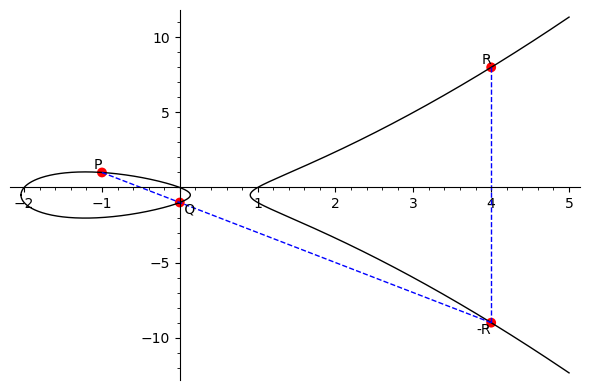
\includegraphics[width=0.8\linewidth]{sage/elliptic_rational_point_addition.png}
    \caption{P + Q na krzywej eliptycznej $y^2+y=x^3-x^2+2x$}
\end{figure}
\par
Definując dodawanie punktów na krzywej eliptycznej w sposób algebraiczny otrzymujemy następujące wzory:
\begin{enumerate}
    \item Przypadek, gdy \( P \neq Q \):
          \begin{align}
              \lambda & = \frac{y_2 - y_1}{x_2 - x_1}, \\
              x_3     & = \lambda^2 - x_1 - x_2,       \\
              y_3     & = \lambda(x_1 - x_3) - y_1
          \end{align}
    \item Przypadek, gdy \( P = Q \):
          \begin{align*}
              \lambda & = \frac{3x_1^2 + a}{2y_1}, \\
              x_3     & = \lambda^2 - 2x_1,        \\
              y_3     & = \lambda(x_1 - x_3) - y_1
          \end{align*}
    \item Szczególny przypadek, gdy \( P = -Q \):
          \begin{align*}
              P + (-P) = \mathcal{O}
          \end{align*}
\end{enumerate}
Dodatkowo odwrotność punktu na krzywej $P$ definujemy jako $-P = (x, -y)$ \cite{Stinson2021}.


\subsubsection{Krzywe eliptyczne na ciele skończonym}
Krzywe eliptyczne zdefiniowane na ciele skończonym $F_p$ oraz $F_{p^n}$ mają kluczowe znaczenie w kryptografii.
W swojej pracy skupiłem się wyłącznie na krzywych zdefiniowanych na ciele skończonym $F_p$ gdzie $p$ jest liczbą pierwszą.
\par
Wykres krzywej eliptycznej nad ciałem $F_p$ nie przypomina krzywej zdefiniowanej na liczbach rzeczywistych.
Krzywa taka składa się z dyskretnych punktów, których współrzędne należą do ciała
na którym jest opisana.
Operacje na krzywej nad ciałem skończonym są zdefiniowane
za pomocą tych samych wzorów algebraicznych, co w przypadku ciała liczb rzeczywistych,
jednak wszystkie działania są wykonywane na ciele $F_p$.
\begin{figure}[!h]
    \centering 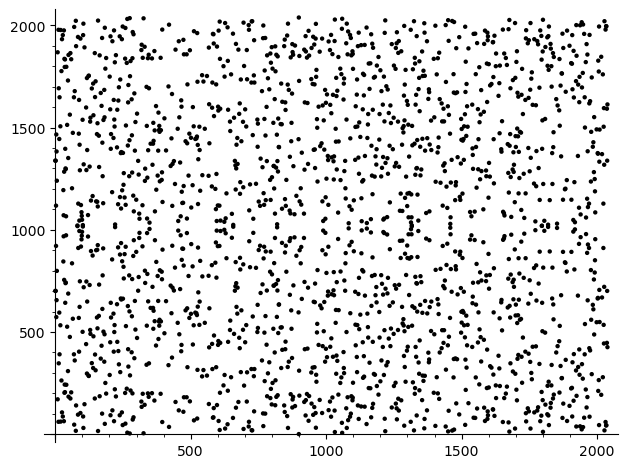
\includegraphics[width=0.8\linewidth]{sage/ec_2_11-9.png}
    \caption{Krzywa eliptyczna $y^2=x^3-4+2$ nad $GF(2^{11} - 9)$}
\end{figure}


\subsubsection{Problem logarytmu dyskretnego}
Problem logarytmu dyskretnego (\textbf{DLP}) jest
podstawą kryptosystemów oparych o grupy.
Jednymi z bardziej znanych są kryptosystem ElGamala oraz protokół wymiany
kluczy Diffie-Hellmana'a.
\\ Problem logarytmu dyskretnego można zdefiniować na grupach cyklicznych.
zarówno na grupie multiplikatywnej $(\mathbb{G},\cdot)$
oraz grupie addytywnej $(\mathbb{G}, +)$, przy odpowiednim zdefiniowaniu działań grupowych.

Jeżeli G jest grupą cykliczną a $\gamma$ jej generatorem, to logarytmem dyskretnym
elementu $\alpha \in G$ nazywamy najmniejszą nieujemną liczbę całkowitą $x$ taką, że:
\[x = \log_{\gamma}{\alpha}\]

Uważa się, że problem logarytmu dyskretnego jest trudny, ponieważ nie istnieje
algorytm, który znajduje $x$ w czasie wielomianowym\cite{Stinson2021}.


\subsubsection{Problem logarytmu dyskretnego na krzywej eliptycznej}
W przypadku krypografii opartej o krzywe eliptyczne, DLP dotyczy cykliczej
grupy addytywnej $(\mathbb{E},+)$ zdefiniowanej na krzywej eliptycznej.
Aby utworzyć taką grupę, wybieramy punkt $P$ na krzywej eliptycznej $\mathbb{E}$,
który będzie generatorem grupy. Wtedy grupa addytywna $\mathbb{E}$ jest generowana przez
kolejne \textit{potęgi} punktu $P$:
\[\ \langle P \rangle = \{P, 2P, 3P, \ldots, nP = \mathcal{O}\}\]
W takim przypadku, ponieważ operacją na grupie jest dodawanie modulo n, to działanie
potęgowania przedstawia się jako zwielokrotnienie punktu $P$:
\[x \cdot P = Q \textrm{ (mod } n)\]
Analogicznie do problemu logarytmu dyskretnego na grupach multiplikatywnych,
problem logarytmu dyskretnego na krzywej eliptycznej polega na znalezieniu
$x$.
\par
Przy odpowiednim wyborze grupy addytywnej, rozwiązanie problemu logarytmu dyskretnego,
tj. znalezienie $x$,
jest trudne \cite{Stinson2021}.


\subsection{Algorytm Rho Pollarda}
 
RYSUNEK LITERKI RHO (bo jak inaczej bez tego mówic o rho pollardzie :))

DODAC OPIS, co się dzieje po znalezieniu kolizji, jak to pozwala obliczyć logarytm dyskretny

CZY TRZEBA opisywać algorym sekwencyjny skoro i tak korzystam z równoległego? Moze samo odesłanie do literatury
\par
DO UZUPEŁNIENIA
\par
\par
Najszybszym znanym algorytmem rozwiązującym problem logarytmu dyskretnego na krzywej eliptycznej
jest algorytm Rho Pollarda,
zaproponowany przez Johna Pollarda w 1978 roku \cite{Pollard1978}.
Pozwala on na znalezienie logarytmu dyskretnego w czasie $O(\sqrt{n})$,
jednak jest to jedynie czas \textit{oczekiwany}, ponieważ ze względu na losową naturę algorytmu \cite{Blake2005}.
W porównaniu do innego znanego algorytmu, Baby-Step Giant-Step \cite{Stinson2021}, algorytm Rho Pollarda jest bardziej
efektywny pamięciowo, nie wymagając
przestrzeni $O(\sqrt{n})$ a jedynie $O(1)$ w wersji sekwencyjnej \cite{Stinson2021}\cite{Blake2005}.
\par
Klasyczny algorytm Rho Pollarda, oparty o poszukiwanie cyklu, słabo się skaluje w przypadku zrównoleglenia,
osiągając jedynie przyśpieszenie rzędu $O(\sqrt{m})$ dla $m$ procesorów \cite{Goldberg}.
Dlatego w swojej pracy wykorzystałem równoległą wersję algorytmu, zaproponowaną przez Van Oorschota i Wienera \cite{Oorschot}.
% \par
% Idea klasycznego algorytmu Rho Pollarda, polega na poszukiwaniu kolizji punktów:
% $$
% X_i = X_{2i}
% $$
% takich, że:
% $$
% X_i = a_i \cdot P + b_i \cdot Q
% $$
% $$
% X_{2i} = a_{2i} \cdot P + b_{2i} \cdot Q
% $$
% Jeżeli znajdziemy kolizję punktów $X_i$ i $X_j$,
% to za pomocą odpowiednich przekształceń możemy obliczyć logarytm dyskretny $x$:
% $$
% a_i \cdot P + b_i \cdot Q = a_j \cdot P + b_j \cdot Q
% $$
% $$
% (a_i - a_j) \cdot P = (b_j - b_i) \cdot Q
% $$
% $$
% x = \frac{b_j - b_i}{a_i - a_j}
% $$

% Zakładając, że $P$ jest generatorem grupy na krzywej eliptycznej, oraz, że chcemy obliczyć logaryytm dyskretny $x$:
% $$
% x\cdot P = Q
% $$
% Idea algorytmu polega na iteracyjnym stosowaniu losowo wyglądającej funkcji $f$, która generuje kolejne trójki
% w postaci $(X_i, a_i, b_i)$, gdzie $X_i$ jest punktem na krzywej eliptycznej, a $a_i$ oraz $b_i$ są liczbami całkowitymi:
% \[
%     f(X, a, b) =
%     \begin{cases}
%         (X + Q,a, b + 1)               & \text{jeśli } X \in S_1, \\
%         (2X, 2a, 2b) & \text{jeśli } X \in S_2, \\
%         (X + P, a+1, b)                           & \text{jeśli } X \in S_3,
%     \end{cases}
% \]

\subsubsection{Równoległy algorytm Rho Pollarda}
Równoległa wersja algorytmu Rho Pollarda, zakłada zastosowanie wielu równoległych ścieżek błądzenia.
\par
Jednostki obliczeniowe poszukują wtedy specalnych punktów nazywanych wyróźnionymi,
które następnie są przekazywane do centralnego serwera w celu znalezienia kolizji między nimi.
\par
Ponieważ sprawdzenie, czy punkt jest wyróźniony następuje w każdej iteracji,
ważne jest aby kryterium decydujące o uznaniu punktu za wyróźniony, było możliwie
szybkie do sprawdzenia.
Często stosowaną metodą, jest sprawdzanie ilości zer na początku lub na końcu binarnej reprezentacji współrzędnej $x$.
\par
Adding walk zakłada jedynie wykonywanie kolejnych operacji dodawania punktów.

Niech $W_0$ będzie punktem startowym, a $f$ funkcją haszującą $f: \langle P \rangle \rightarrow \{1,..s\}$ o możliwie jednostajnym rozkładzie.
Następnie, potrzebujemy tablicy wstępnie obliczonych punktów:
$R_i = c_i P + d_i Q$ dla $0 \leq i \leq s - 1$.
Funkcja iteracyjna jest wtedy zdefiniowana w następujący sposób:
$$
    W_{i+1} = W_i + R_{f(W_i)}
$$
Ważną kwestią jest też rozmiar tablicy z punktami wstepnie obliczonymi.
Zbyt mały rozmiar powoduje, że funkcja nie będzie dostatecznie losowa.
W eksperymentach praktycznych pokazano, że dla $s \geq 16$, funkcja zapewnia
wystarczający poziom losowości,  niezależnie od rozmiaru grupy.
 \cite{Teske2000}
\par
Istotną zaletą tej funkcji w przypadku programu uruchamianego na GPU,
jest uniknięcie rozgałęzień podczas każdej iteracji, co jest szczególnie istotne w przypadku architektury SIMD.
Prawie zawsze wykonujemy tą samą operację dodawania dwóch punktów,
poza mało prawdopodobnym przypadkiem w którym $W_i == R_{f(W_i)}$.
\par
\newpage
% \newpage % Zaleca się otwieranie rozdziału od nowej strony.
\section{State~of~Art}
\label{sc:state}

\subsection{GPU}
Procesory graficzne są dedykowane do wykonywania wielu równoległych obliczeń.
Dzięki temu, są bardzo wydajne w zadaniach które można łatwo zrónoleglić.
Wiele algorytmów do kryptoanalizy pozwala na przetwarzanie równoległe, 
w szczególności algorytm \textbf{rho-Pollarda}.
\subsubsection*{Solving Discrete Logarithms in Smooth-Order Groups with CUDA}
W roku 2012 na karcie graficznej NVIDIA Tesla M2050 osiągnięto wydajność na poziomie
51.9 miliona operacji mnożenia modularnego 768-bit na sekundę.
Implementacja opierała się głównie na języku C z CUDA framework wraz z jednostkowymi segmentami
w języku PTX który jest zbiorem instrukcji dla CUDA GPU.
Praca ma dla mnie szczególną na tym etapie, ponieważ razem z pracą udostępniono kod
implementacji na prawach open-source, dodatkowo opisuje
ograniczenia i założenia jakie należy uwzględnić przy implementacji
algorytmu rho-Pollarda na GPU\cite{henry-goldberg-cuda}.

\subsubsection*{ECC2K-130 on NVIDIA GPUs}
Artykuł opisuje implementację algorytmu rho-Pollarda na karcie graficznej NVIDIA 
GTX 295.
Autorzy wybrali krzywą Koblitza ECC2K-130.
Opisano decyzje związane z wyborem bazy ( w tym przypadku wybrano bazę normalną).
Przedstawiono również szczegóły związane z zarządzaniem pamięcią oraz problem związany
z DRAM'em karty (przy pełnej utylizacji GPU w pamięci brakowało miejsca na input)
Wynik: Średnio obliczenie ECDLP na tej krzywej zajełoby 2 lata przy 534 kartach.

\subsection{FPGA}
\subsubsection*{Solving Discrete Logarithms in Smooth-Order Groups with CUDA}
W 2014 opublikowano pracę przedstawiającą implementację FPGA
na platformie Virtex-6.
dedykowaną do rozwiązania logarytmu dyskretnego na 113-bitowej krzywej Koblitza.
Opisano zastosowane zabiegi poprawiające optymalizację, oraz design
poszczególnych moduł
Na przykład w celu lepszej optymalizacji, wykorzystano bazę normalną
$F_{2^m}$ w jednym z modułów do liczenia automorfizmu punktów.
Wynik po ekstrapolacji to 28 dni na rozwiązanie logarytmu na krzywej Koblitza 113 bit.

\subsection{CPU}
CPU nie są najwydajniejszą architekturą do wykonywania równoległych obliczeń.
Zazwyczaj charakteryzują się znacznie wydajniejszymi jednostkami obliczeniowymi (rdzeniami)
niż na przykład GPGPU, ale jest ich również znacznie mnniej niż w GPGPU.
CPUs są najlepiej przystosowane do przetwarzania potokowego.
\subsubsection*{A Review on solving ECDLP over Large Finite Field using Parallel
	Pollard's Rho (p) Method}
Praca przedstawia wyniki czasowe przy obliczaniu ECDLP na
ciele skończonym rzędu p do 85-bitów.
Zastosowano do tego cluster CPU o 256 rdzeniach octa-core.
Artykuł również jest interesujący ponieważ zwięźle opsuje background matematyczny
oraz przejrzyście przedstawia wersję równoległą
algorytmu rho Pollarda\cite{rewiev-elliptic-cpu}.
Wynik to 52 godziny dla krzywej na ciele rozmiaru p = 85-bitów.



\newpage
\section{Implementacja}
Ta część pracy jest poświęcona implementacji całego systemu,
wraz ze szczegółowym opisem narzędzi oraz sprzętu wykorzystanego
przy pracy nad projektem.
\par
Większość opisanych zagadnień dotyczy części klienta napisanej w CUDA C++,
poza sekcją na końcu, poświęconą serwerowi oraz częsci klienta działającej na CPU.

\subsection{Narzędzia oraz sprzęt}
\subsubsection{Sprzęt}
\begin{itemize}
    \item OS: openSUSE Tumbleweed 20240812
    \item CPU: Intel Core i5-10600KF 4.10 GHz
    \item RAM: 16 GB
    \item GPU: GeForce RTX 2070 Super
\end{itemize}

\subsubsection{Program po stronie CPU}
Implementacja programu serwera działającego po stronie CPU, została wykonana z wykorzystaniem
języka Python w wersji 3.11.1 wraz z pakietem obliczeniowym SageMath w wersji 10.4.beta3.
Program klienta został zaimplementowany z wykorzystaniem języka Python w wersji 3.11.1 oraz
języka CUDA C++ w wersji 12.4.

\subsubsection{System budowania oraz kompilacja CUDA C++}
W celu zarządzania kompilacją częsci projektu napisanej w języku CUDA oraz C++,
wykorzystałem narzędzie \textit{CMake}.
\textit{CMake} zapewnia natywne wsparcie dla języka CUDA,
co znacznie upraszcza wszelkie zarządzanie kompilacją oraz linkowanie.
Dodatkowo, wymaga to znacznie mniej wstępnej konfiguracji niż analogiczne
rozwiązanie z wykorzystaniem samego narzędzia do budowania takiego jak \textit{Make} lub \textit{Ninja}.
\par
Program napisany w CUDA kompilowany był z wykorzystaniem kompilatora NVCC dostarczonego wraz z pakietem
\textit{CUDA Toolkit} w wersji 12.4.
NVCC do kompilacji kodu po stronie host'a (CPU) wykorzystuje kompilator z GCC w wesji 13.3.1.


\subsubsection{Testy}
Wszelkie testy poprawności implemetnacji rozwiązania są przeprowadzane z wykorzystaniem framework'a PyTest dla języka Python.
Python wraz z wykorzystaniem pakietu obliczeniowego SageMath generuje testowe dane, które
są przekazywane do programu działającego na GPU. Następnie, otrzymane wyniki są porównywane z rezultatami
obliczonymi przy wykorzystaniu SageMath. Wykorzystanie PyTest oraz SageMath znacznie przyśpieszyło pracę
nad implementacją operacji na krzywej eliptycznej oraz docelowej implementacji algorytmu Rho Pollarda.
Możliwość szybkiego generowania dużych zbiorów danych testowych, pozwoliło na wczesne zauważenie wielu subtelnych błędów
na etapie implementacji.



\subsection{Artmetyka na ciele $F_{p}$}
\subsubsection{Reprezentacja długich liczb}
Natywnie w języku C oraz CUDA C++ nie istnieje typ danych, który pozwalałby na przechowywanie liczb większych niż 64 bitowe.
W celu przeprowadzenia obliczeń na liczbach większych niż natywny rozmiar słowa bitowego,
niezbędna jest odpowiednia implementacja nowych typów danych jak i samych operacji.
W przypadku ciała $F_{p}$, gdzie $p$ jest liczbą pierwszą o rozmiarze 79 bit, potrzebujemy conajmniej 79 bitowego typu danych, do samego przechowywania liczb.
Jednak nawet 79 bitowy typ danych nie wystarczy, jeżeli chcemy przeprowadzić operację mnożenia
dwóch liczb 79 bitowych. W takim przypadku, wynik pośredni może być maksymalnie $2*79 = 158$ bitowy.
Dodatkowo, w celu reprezentacji takiej liczby, nie możemy się posłużyć wektorem składającym się z największego
dostępnego natywnie typu danych,
ponieważ wyniki pośrednie z operacji mnożenia lub dodawania mogą przekroczyć rozmiar słowa bitowego.
W tym celu musimy wykorzystać typ danych mniejszy od maksymalnego. W przypadku CUDA C++, największy wspierany typ danych
wynosi 64 bit, więc w celu reprezentacji liczb, musiałem wykorzystać wektor składający się z 32 bitowych słów.
Najbliższa wielokrotność liczby 32 bitowej, większa niż 158 bit to 160 bit,
dlatego w celu reprezentacji liczb na ciele, wykorzystywany jest wektor postaci:
$$
    \sum_{i = 0}^{4} x_i\cdot 2^{32}
$$

Zaimplemetowany jako tablica typu u\_int32:
\begin{lstlisting}[language=C++]
struct bn
{
    uint32_t array[5];
};
\end{lstlisting}
Dla liczb, na których bezpośrednio nie będą wykonywane operacje arytmetyczne, wykorzystywany jest mniejszy, tymczasowy typ
danych.
Ograniczone zasoby szybkiej pamięci współdzielonej na GPU, wymuszają oszczędne zarządzanie pamięcią. W celu
przechowywania wstępnie obliczonych punktów w pamięci współdzielonej, wykorzystuję następujący typ danych:
\begin{lstlisting}[language=C++]
struct small_bn
{
    uint32_t array[3];
};
\end{lstlisting}
\par
Liczby w takiej postaci, przed przeprowadzeniem na nich operacji arytmetycznych, są ładowane z pamięci współdzielonej i z powrotem konwertowane na większy typ danych.
Pozwala to zaoszczędzić $ 2 \cdot 32$ bitów na każdej liczbie, co w przypadku punktu składającego się z dwóch wspórzędnych
daje oszczędnośc $2 \cdot 2 \cdot 32 = 128$ bitów na punkt znajdujący się w pamięci.

\subsubsection{Operacje na długich liczbach}
Do operacji na długich liczbach, odpowiednio dostosowałem małą bibliotekę
dostępną w domenie publicznej: \textit{tiny-bingum-c}.
Bilbioteka ta dostarcza podstawowe operacje na dużych liczbach w postaci wektorów, takie jak dodawanie, odejmowanie, mnożenie czy dzielenie.
Wykorzystuje w tym celu standardowe algorytmy \cite{Menezes2001} wykorzystywane przy obliczeniach \textit{multiple precision}.
Dużą zaletą ten biblioteki jest jej prostota i brak wykorzysywania standardowej biblioteki C oraz dynamicznej alokacji pamięci.
Wszystkie operacja są wykonywane z wykorzystaniem stosu,
co pozwala na jej wykorzystanie w środowiskach takich jak GPU, gdzie dostęp do dynamicznej alokacji pamieci jest ograniczony.
W większości przypadków, aby dostosować kod z biblioteki do CUDA C++ wystarczyło dodanie
odpowiedniej dyrektywy \textit{\_\_device\_\_} przed każdą deklaracją funkcji, która informuje kompilator, że dana funkcja
będzie wykonywana na GPU.
\par
Prymitywy matematyczne dostarczane przez bibliotekę \textit{tiny-bignum-c} nie są jednak wystarczające do przeprowadzenia
operacji na ciele $F_{p}$.
W związku z tym, zaimplementowałem dodatkowe operacje modularne takie jak mnożenie, dodawanie, odejmowanie i odwrotność modulo.

\subsubsection{Dodawanie i odejmowanie modulo}
Dodawanie oraz odejmowanie modulo $p$, wygląda bardzo podobnie do standardowego dodawania i odejmowania.
\par
W przypadku odejmowanie dówch liczb na ciele $F_{p}$, nie ma potrzeby redukcji modulo p po każdej operacji.
Jednak niezbędne jest upewnienie się, że wynik nie jest ujemny. Ponieważ prowadzimy obliczenia na liczbach bez znaku,
to w sytuacji gdy $a - b = c; a < b$, nastąpi przepełnienie i wynik będzie w postaci $2^{32 \cdot n}-1 - c$, gdzie $n$ to rozmiar
wektora do przechowywania liczb. Na szczęście, możemy bardzo łatwo wrócić do poprawnego wyniku wykorzystując jedną operację
dodawania. Korzystając z faktu, że wszystkie podstawowe operacje są wykonywane modulo $2^{32 \cdot n}$:
$$
    2^{32 \cdot n} - 1 - c + p \equiv p - c \pmod{2^{32 \cdot n}}
$$
Przykładowa implementacja z wykorzystaniem \textit{tiny-bignum-c}:

\begin{lstlisting}[language=C++]
bignum_sub(a, b, c);
if (bignum_cmp(a, b) == SMALLER)
{
    bignum_add(c, p, temp);
    bignum_assign(c, temp);
}
\end{lstlisting}
\par
Dodawanie modulo $p$ jest prostsze.
Aby wykonać dodawanie modularne, wystarczy wykonać standardowe dodawanie i ewentualnie jeżeli $a + b >= p$ zredukować wynik odejmując
od niego liczbę p.

\subsubsection{Mnożenie modulo}
Mnożenie modularne jest bardziej kosztowne niż dodawanie czy odejmowanie, ponieważ wymaga dzielenia z resztą.
W swojej pracy przeprowadzam standardowe mnożenie modularne, jednak również istnieją bardziej wydajne sposoby, na przykład wykorzystanie redukcji Barreta CITE APPLIED.
\par
Aby przeprowadzić klasyczne mnożenie modularne ciele $F_{p}$, na początku musimy przeprowadzić standardowe mnożenie długich liczb.
Następnie, otrzymany wynik dzielimy przez $p$ i zwracamy resztę z dzielenia.
Zarówno mnożenie jak i dzielenie z resztą, są funkcjami dostarczonymi
w bibliotece \textit{tiny-bignum-c}, więc mnożenie modularne sprowadza się do wykonania tych dwóch operacji jedna po drugiej.

\subsubsection{Odwrotność modulo}
Obliczanie odwrotności modulo $p$ jest najbardziej kosztowną operacją na ciele $F_{p}$, głównie ze względu
na wielokrotne dzielenie w pętli.
Algorytm obliczania odwrotności modulo $p$ zaimplementowałem z wykorzystaniem rozszerzonego algorytmu Euklidesa,
który został zmodyfikowany do działania na liczbach nieujemnych. Główna różnica względem klasycznego algorytmu,
polega na wykorzystaniu dodatkowych zmiennych do śledzenia zmian znaku wyniku.

\begin{algorithm}[]
    \caption{Odwrotność modularna a mod b}
    \label{alg:inverse}
    \begin{algorithmic}[1]
        \State \text{\textbf{Input: }} $a, b$
        \State $b_0 \gets b$
        \State $x_0 \gets 0$
        \State $x_1 \gets 1$
        \State $x_{0\_sign} \gets 0$
        \State $x_{1\_sign} \gets 0$

        \While{$a > 1$}
        \State $q \gets a \div b$
        \State $t \gets b$
        \State $b \gets a \mod b$
        \State $a \gets t$

        \State $t_2 \gets x_0$
        \State $t_{2\_sign} \gets x_{0\_sign}$
        \State $qx_0 \gets q \times x_0$

        \If{$x_{0\_sign} \neq x_{1\_sign}$}
        \State $x_0 \gets x_1 + qx_0$
        \State $x_{0\_sign} \gets x_{1\_sign}$
        \Else
        \If{$x_1 > qx_0$}
        \State $x_0 \gets x_1 - qx_0$
        \State $x_{0\_sign} \gets x_{1\_sign}$
        \Else
        \State $x_0 \gets qx_0 - x_1$
        \State $x_{0\_sign} \gets 1 - x_{0\_sign}$
        \EndIf
        \EndIf

        \State $x_1 \gets t_2$
        \State $x_{1\_sign} \gets t_{2\_sign}$
        \EndWhile
        \If{$x_{1\_sign} == 1$}
        \State \Return $b - x_1$
        \Else
        \State \Return $x_1$
        \EndIf

    \end{algorithmic}
\end{algorithm}


\subsubsection{Biblioteka CGBN}
W pierwotnej wersji swojej pracy, do operacji na dużych liczbach wykorzystałem specjalną bibliotekę CGBN dla platformy CUDA. Oferuje ona
wszystkie podstawowe operacje na długich liczbach, takie jak dodawnia, odejmowanie czy mnożenie nawet do 32 tyś. bitów.
Dodatkowo, posiada ona implementację bardziej zaawansowanych funkcji, takich jak odwrotność modulo czy redukcja Barreta.
Niestety, biblioteka ta narzuca spore ograniczenia pod kątem zasobów. Niezbędne jest grupowanie wątków w grupy
4, 8, 16 lub 32. Wysoką wydajność obliczeń, uzyskiwałem dopiero w grupach składających się z 32 wątków.
Pomimo znacznie szybszego wykonywania się poszczególnych operacji w ramach takiej grupy wątków, narzucone
ograniczenia oraz wysokie użycie rejestrów uniemożliwiało
efektywne zaimplementowanie dużej ilości takich instancji działających równolegle.
Całkowita wydajność mierzona w ilości operacji na krzywej na sekundę osiągnięta z jej wykorzystaniem była średnio 4.57 razy gorsza, niż
z wykorzystaniem znacznie prostszej implementacji na bazie \textit{tiny-bignum-c}.


\subsection{Funkcja iterująca}
DO UZUPEŁNIENIA - max 0.5 strony - ogólnie przypomnienie tego co było na początku w teorii, że addition walk jest lepszy dla SIMD niż klasyczna wersja rho pollarda


\subsubsection{Wstępnie obliczone punkty}
Dostęp do wstępnie obliczonych punktów jest niezbędny w każdej iteracji \textit{Addition walk}.,
dlatego ważne jest, aby je przechowywać w szybkiej pamięci. Wykorzystałem w tym celu pamięć współdzieloną \textit{shared memory}.
W przeciwieństwie do znacznie większej pamięci globalnej, jest ona przechowywana bezpośrednio na SM \cite{CUDA_BOOK}.
Ponieważ ilość punktów która zapewnia dostatecznie losowy spacer po krzywej eliptycznej jest stosunkowo niewielka \cite{Teske2000},
to rozmiar pamięci nie stanowi problemu. W docelowej wersji, przechowywane jest 128 punktów.
\par
Funkcja przydzielająca punkt wstępnie obliczony, na podstawie aktualnie sumowanego punktu została zaimplementowana
poprzez operację AND maski bitowej ze współrzędną $x$ punktu.
W ten sposób, każdy punkt $W_i$ jest przyporządkowany do jednego z 128 wstępnie obliczonych punktów,
a następnie punkty są dodawane do siebie.


\subsubsection{Punkty wyróżnione}
W ramach każdej iteracji, musimy w wydajny i szybki sposób sprawdzić, czy obliczony punkt jest punktem wyróźnionym.
W mojej implementacji, kryterium warunkującym jest liczba zer na końcu współrzędnej $x$ obliczonego punktu.
\par
Do sprawdzenia, czy punkt jest wyróźnionym, słuzy prosta funkcja obliczająca bitową operację AND ze
współrzędnej punktu oraz specjalnej maski bitowej wyznaczanej na podstawie poszukiwanej ilości zer.
Przykładowo, dla poszukiwanej liczby zer 3, maska będzie w postaci $0 ... 00111$. Jeżeli
również ostatnie 3 bity współrzędnej $x$ będzie miało zerowy znak, to otrzymany wynik operacji AND wyniesie 0.
\par
Istotne jest, aby taka sama funkcja została zaimplementowana po stronie serwera na CPU, ponieważ w przypadku znalezienia kolizji,
musi on być w stanie odtworzyć cały spacer losowy prowadzący do danego punktu wyróźnionego.

\begin{algorithm}
    \caption{Funkcja \texttt{is\_distinguish}}
    \begin{algorithmic}[1]
        \State \textbf{Input:} $x$, $liczba\_zer$
        \State $mask \gets 1 \ll liczba\_zer - 1$

        \If{$(x \ \& \ mask) == 0$}
        \State \Return \textbf{true}
        \Else
        \State \Return \textbf{false}
        \EndIf
    \end{algorithmic}
\end{algorithm}

\par
Aby ułatwić testy na różnych etapach implementacji całego systemu,
liczba sprawdzanej ilości zer jest sparametryzowana. Przy starcie każdej serii obliczeń, poszukiwana liczba zer jest jednym z parametrów przekazywanym
do funkcji kernel'a.
\par
Po znalezieniu punktu wyróźnionego, ustawiana jest specjalna flaga w strukturze przechowującej dane punktu oraz
jest on zapisywany pod pierwsze wolne miejsce w pamięci globalnej.

\subsubsection{Dodawanie punktów na krzywej eliptycznej}
DO UZUPEŁNIENIA - max 0.5 strony większość jest poniżej.
MOZE NAWET POMINĄC, w sumie to przepisanie tego co jest w teorii z wykorzystaniem zaimplementowanych prymitywów matematycznych???
\subsubsection{Obliczanie odwrotnosci w seriach}
Każda operacja dodawania punktów na krzywej eliptycznej we współrzędnych afinicznych, składa się z 3 mnożeń modularnych oraz jednej operacji obliczania odwrotności w ciele.
Przeprowadza się również operację dodawania i odejmowania modularnego, jednak ich koszt obliczeniowy jest pomijalnie mały \cite{Blake2005}.
\par
Koszt dodawania punktów na krzywej:
$$
    1O + 3M
$$
Najdroższym działaniem, które wpływa na wysoki koszt obliczeniowy  mnożenia modularnego oraz odwrotności w ciele,
jest operacja dzielenia \cite{Menezes2001}.
Przykładowo, wykorzystywana przeze mnie implementacja dzielenia stosuje prosty algorytm \textit{long division},
o złożoności obliczeniowej $O(n^2)$.
\par
Warto zauważyć, że operacja obliczania odwrotności modularnej z wykorzystaniem algorytmu euklidesa, wykonuje dzielenie
podczas obliczania modulo, na każdym etapie pętli wewnątrz algorytmu \ref{alg:inverse}.
To czyni ją najdroższą operacją na ciele, znacznie kosztowniejszą niż operacja mnożenia modularnego.
\par
Aby przyśpieszyć obliczenia, zastosowałem technikę obliczania wielu odwrotności za jednym razem,
znaną jako \textit{Montgomery Trick} \cite{Montgomery1987}.
\par
Idea stojąca za tym sposobem, jest następująca.
Niech $x_1, \cdots ,x_n$ będą elementami, których odwrotność chcemy policzyć.
Na początku obliczamy tablicę elementów, w postaci $a_1 = x_1, a_2 = x_1\cdot x_2 , \cdots, a_n = x_1 \cdots x_n$.
Następnie, obliczamy odwrotność ostatniego elementu $a_n$ za pomocą jednej operacji odwrotności w ciele.
Teraz, aby policzyć odwrotność elementu $x_n$ wystarczy wykonać jedynie operację mnożenia
$b_n = a_{n-1} \cdot a_{n}^{-1}$. Kolejne elementy obliczamy analogicznie, za pomocą mnożenia:
$b_{n-1} = a_{n-2} \cdot b_{n}$.
\textit{Montgomery trick} pozwala na zamianę:
$$
    nO = O + 3(n - 1)M
$$
\par
Sposób implementacji tej tej metody wymagał podjęcia paru decyzji.
Pierwszym problemem który pojawia się w metodzie Montgomerego,
jest konieczność
obliczania iteracji dla wielu punktów jednocześnie.
\par
Jednym ze sposobów by tego dokonać,
jest zsynchronizowanie wielu wątków w ramach bloku obliczeniowego, a następnie przekazanie
jednemu z nich, za pomocą pamięci współdzielonej, wszystkich liczb do obliczenia odwrotności.
Następnie, wątek zwracałby obliczone odwrotności za pomocą pamięci współdzielonej.
Jak zauważono w pracy \cite{Boss2015}, takie podejście nie jest optymalne w przypadku GPU.
Wymagałoby to sporo synchronizacji pomiędzy wątkami, oraz sporej ilości zapisów i odczytów
z pamięci współdzielonej, która pomimo bycia znacznie szybszą niż pamięć globalna, nie jest tak
szybka jak prywatna pamięc w postaci rejestrów. Dodatkowo, z racji, że tylko jeden
wątek oblicza odwrotności, pozostałe muszą bezczynnie czekać.
\par
Dlatego sposobem, który zastosowałem jest obliczanie wielu odwrotności
w ramach jednego wątku. Oznacza to, że każdy wątek zamiast przetwarzać tylko jeden punkt startowy,
dostaje ich $n$ na początku działania programu.
\par
\textit{Naiwne} podejście polegałoby na przekazaniu każdemu z wątków $n$ punktów startowych,
i oczekiwanie aż znajdzie dla każdego punktu startowego odpowiadający mu punkt wyróźniony. Taki sposób powoduje,
że bardzo szybko zaczynamy tracić zyski z metody Montgomerego, a nawet zaczynamy działać wolniej,
z powodu dodatkowych obliczeń, których nie wykorzystujemy.
Wynika to z faktu,
że po znalezieniu $i$ punktów, zysk z metody jest postaci:
$$
    (n-i)O = O + 3(n-i)M + 3(i)M
$$
Gdzie $3(i)M$ to mnożenia, które nie przyczyniają się do znalezienia nowych punktów wyróźnionych, więc należy je traktować jako niepotrzebne spowolnienie.
\par
W celu rozwiązania tego problemu, zastosowałem okienkowanie obliczeń w tablicy o stałym rozmiarze $m$.
Sposób ten wymaga, aby każda wątek otrzymał $n > m$ punktów startowych w wyznaczonym dla niego miejscu w pamięci globalnej.
Im większa różnica $n-m$ tym lepszy
stosunek czasu obliczeń do narzutu czasowego związanego ze startem programu.
\par
Na początku działania wątku, ładujemy do tablicy okna kolejne $m$ punktów startowych z pamięci globalnej.
Następnie w pętli obliczamy odwrotności wymagane dla operacji dodawnia punktów i przeprowadzamy dodawanie. Tym sposobem,
w jednym kroku pętli, wykonujemy jedną iterację algorytmu Rho Pollarda dla $m$ punktów. Na samym końcu każdego kroku pętli,
sprawdzamy czy każdy z nowo obliczonych punktów, czy jest punktem wyróźnionym. Jeżeli tak,
znaleziony punkt zapisujemy na pierwszym wolnym miejscu w pamięci globalnej, a na jego miejsce ładujemy do tablicy
okna kolejny punkt startowy.
Dzięki temu, przez większość czasu obliczeń, wykorzystujemy pełny zysk z metody Montgomerego.
\par
Jeżeli dodatkowo zastosujemy flagę, która kończy obliczenia wszystkich wątków w bloku, gdy pierwszy wątek,
znajdzie $n-m$ punktów wyróźnionych, to otrzymujemy maksymalny poziom wydajności w ciągu całej fali obliczeń.
Efekt ten jest dokładniej opisany w części poświęconej problemowi \textit{tailing effect}.
\par
Wzrost wydajności mierzony w ilości operacji dodawania punktów na krzywej na sekundę, który udało mi się osiągnąć, wynosi około 90\% względem wersji, która nie wykorzystuje
metody Montgomerego.




% schemat
\begin{figure}[H]
    \centering
    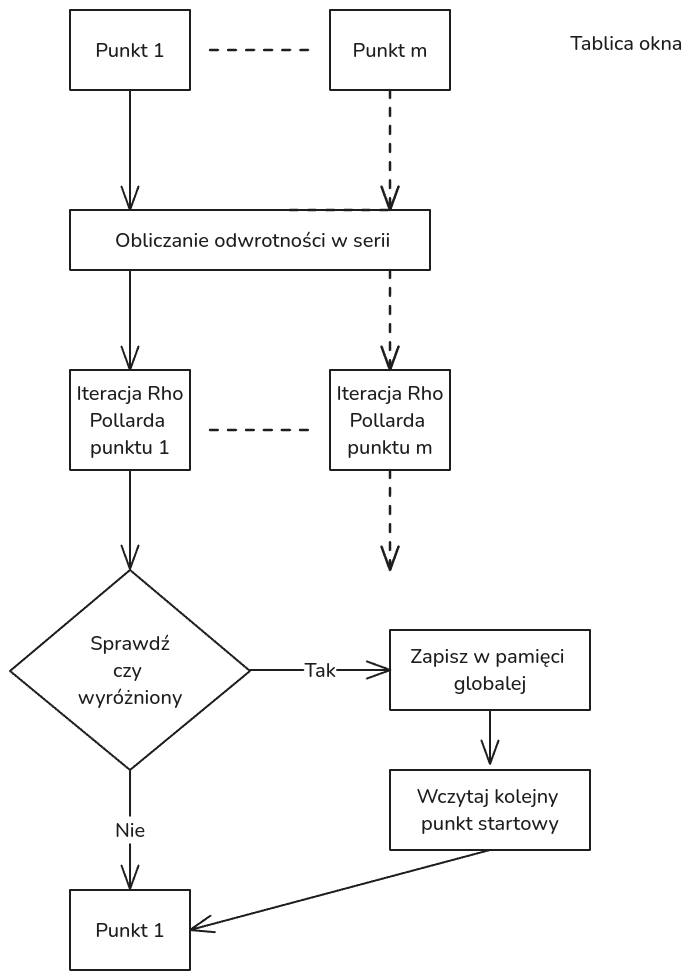
\includegraphics[width=0.8\textwidth]{img/okienkowanie_3.png}
    \caption{Schemat działania pojedyńczego kroku w pętli z wykorzystaniem okienkowania}
    \label{fig:windowing}
\end{figure}

\begin{table}[h!]
    \centering
    \begin{tabular}{|c|c|c|}
        \hline
        \textbf{Wielkość okna} & \textbf{Średnia ilość operacji na sekundę} & \textbf{Wzrost wydajności (\%)} \\ \hline
        Brak                   & 1000                                       & 0\%                             \\ \hline
        5                      & 1500                                       & 25\%                            \\ \hline
        10                     & 1700                                       & 30\%                            \\ \hline
        15                     & 1900                                       & 35\%                            \\ \hline
        20                     & 2100                                       & 40\%                            \\ \hline
    \end{tabular}
    \caption{Porównanie algorytmu z metodą Montgomery DANE NA RAZIE W FORMIE PLACEHOLDERA, NIE ZDAZYLEM PRZESZUKAC LOGOW W POSZUKIWANIU DOKLADNYCH WYNIKOW, ale coś około 96 milionów vs 56 milionów dla okna rozmiaru 10}
    \label{tab:comparison}
\end{table}


\subsection{Tail effect}
Tail Effect to zjawisko, które polega na nierównomiernym obciążeniu wątków na GPU.
W przypadku równoległej wersji algorytmu Rho Pollarda, to zjawisko jest szczególnie widoczne,
ze względu na losowość funkcji błądzenia po krzywej.
Wątki znajdują punkty wyróżnione w różnym, losowym czasie.
\par
Po znalezieniu punktu wyróżnionego, wątek musi zaczekać, na zakończenie pracy wszystkich
pozostałych wątków w ramach jednego bloku.
To powoduje, że tylko przez krótki czas są wykorzystywane wszystkie zasoby GPU.
\par
Jednym ze sposobów na zmniejszenie tego efektu, jest wydłużenie czasu pracy każdego z wątków poprzez zwiększenie ilości punktów wyróżnionych,
które musi znaleźć. Dzięki temu spada prawdopodobieństwo, że zakończy on swoją pracę znacznie wcześniej niż pozostałe wątki w bloku.
Zastosowanie metody z oknem, opisanej w poprzedniej sekcji, pozwala na znacznie lepszą utylizację zasobów przez większość
czasu obliczeń.
\par
Rys \ref{fig:tail_effect_1} oraz \ref{fig:tail_effect_3} przedstawiają czas pracy każdego z wątków w bloku, w trakcie jednej fali obliczeń.
W trakcie testu, każdy z wątków poszukiwał punktów wyróżnionych z 17 zerami na końcu współrzędnej $x$. Widoczne jest
znaczne lepsze wykorzystanie zasobów GPU w przypadku, gdy każdy z wątków musi znaleźć 3 punkty wyróżnione przed zakończeniem pracy.
Zmniejsza to wplyw anomalii, gdy punkt wyróżniony jest znajdowany znacznie wcześniej lub później niż wynika z wartości oczekiwanej.

% wykres
\begin{figure}[H]
    \centering
    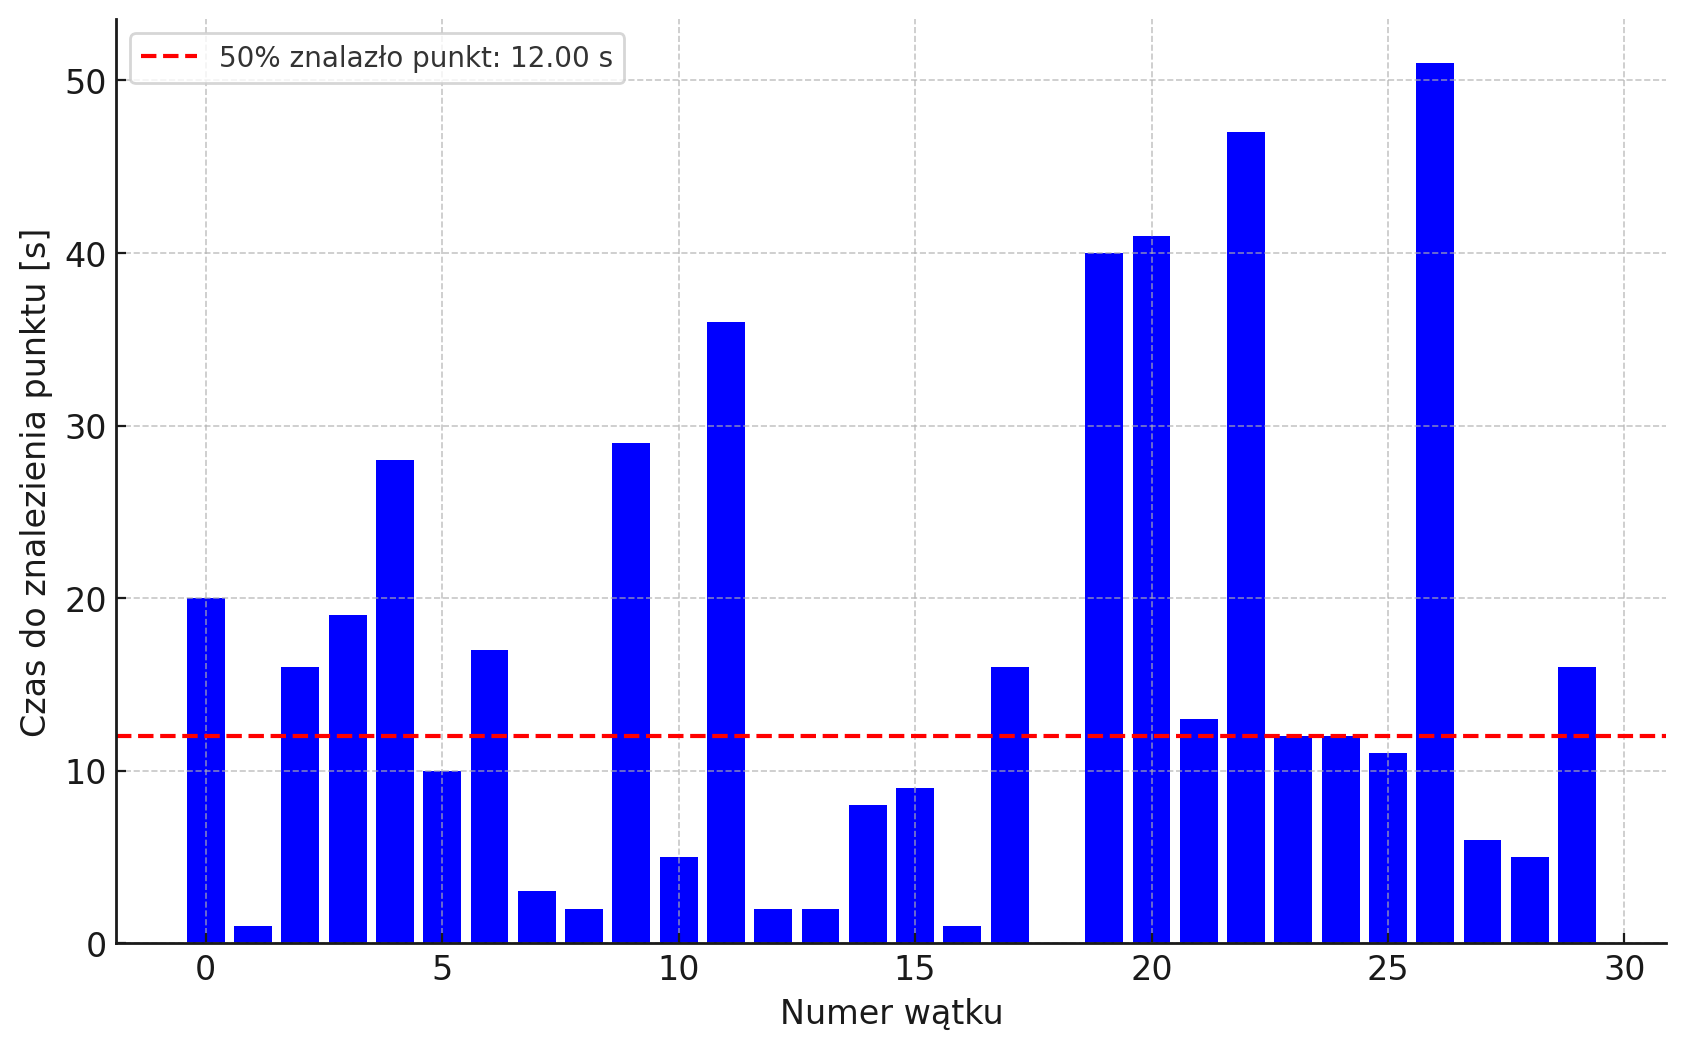
\includegraphics[width=1\textwidth]{img/tailing_effect_single_17.png}
    \caption{Tail effect widoczny na małej grupie wątków. Wątki kończą pracę po znalezieniu jednego punktu wyróżnionego.
        Większość czasu obliczeń, jest wykorzystywana tylko przez małą liczbę wątków.}
    \label{fig:tail_effect_1}
\end{figure}

% wykres
\begin{figure}[H]
    \centering
    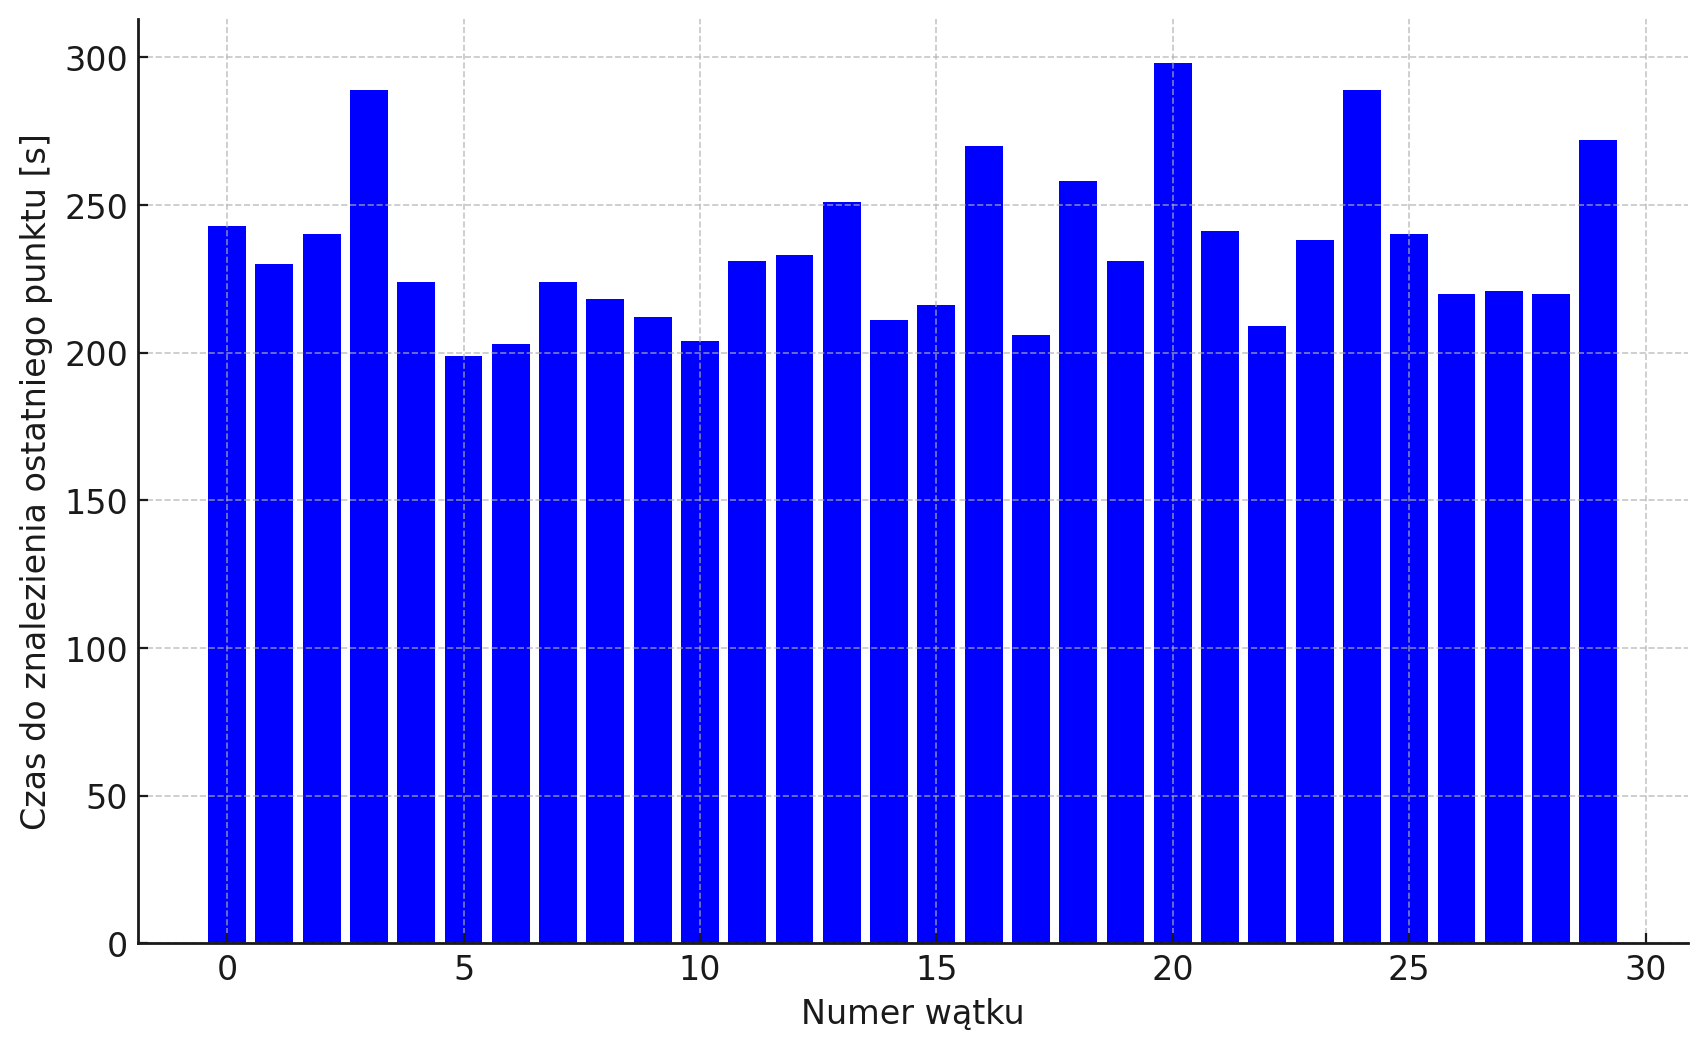
\includegraphics[width=1\textwidth]{img/tailing_effect_3_17.png}
    \caption{Tail effect widoczny na małej grupie wątków. Wątki kończą pracę po znalezieniu 3 punktów wyróżnionych.
        Widoczne jest znacznie lepsze wykorzystanie zasobów GPU, przez większość czasu obliczeń.}
    \label{fig:tail_effect_3}
\end{figure}

\par
Aby jeszcze bardziej zniwelować efekt, zastosowałem specjalną flagę w pamięci współdzielonej, która pozwala zakończyć obliczenia wszystkich wątków w bloku,
po tym, jak pierwszy z nich znajdzie wszystkie punkty wyróżnione. Pozwala to zwolnić miejsce na kolejny blok
i pozwolić na załadowanie nowych danych do obliczeń, gdy tylko poziom wykorzystania zasobów zacznie spadać.
Karty graficzne z architekturą Turing,
pozwalają na kolejkowanie wielu uruchomień kernel'a wykorzystując mechanizm strumieni CUDA.
Dzięki wykorzystaniu strumieni, scheduler CUDA
może uruchamiać kolejne bloki obliczeń z kolejki zadań, gdy tylko
zwolni się miejsce na kolejny blok, zamiast czekać ze startem na zakończenie poprzedniego kernel'a \cite{cuda}.
\par
Rys \ref{fig:tail_effect_3} przedstawia wykres sumy znalezionych punków od czasu przy zakolejkowaniu dwóch kernel'i w odzielnych strumieniach.
Widoczne jest przejmowanie przez strumień Stream 2 wolnych zasobów, zwalnianych przez Stream 1.
Wypłaszczenie krzywej sumy punktów pod koniec pracy każdego ze strumieni, jest
efektem ogona, spowodowanym przez nierównomierny czas pracy na poziomie bloków.
Jednak dopóki jest zapewniona zastępowalność bloków na SM, efekt nie wpływa na wydajność obliczeń.



% wykres
\begin{figure}[H]
    \centering
    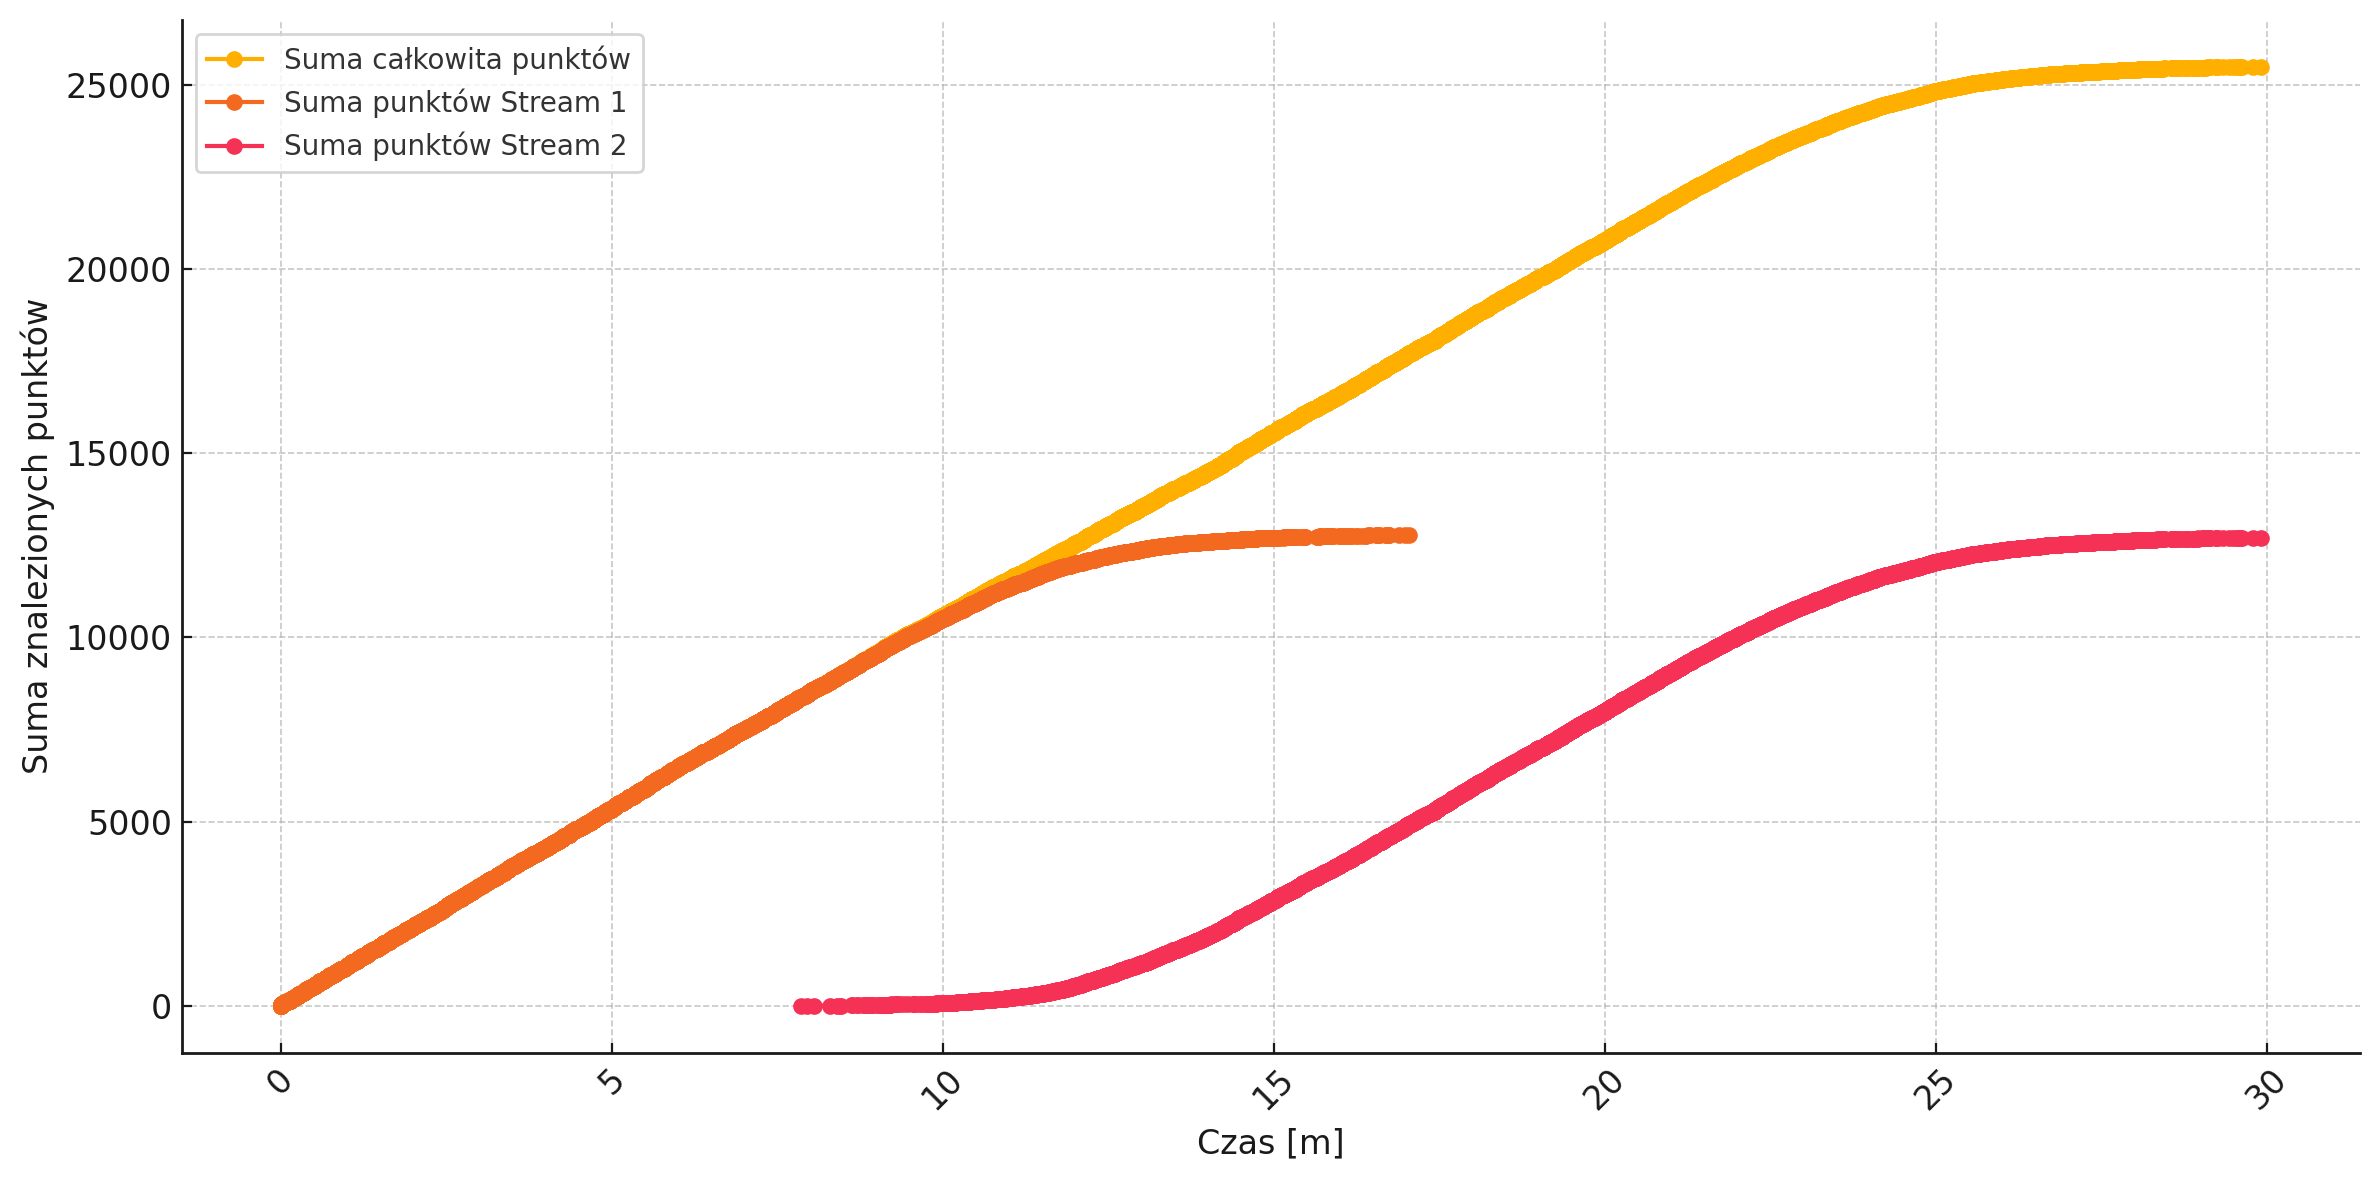
\includegraphics[width=1\textwidth]{img/streams.png}
    \caption{Suma znalezionych punktów wyróżnionych z podziałem na strumienie,
        gdzie każdy z wątków szukał 10 punktów wyróżnionych z 22 zerami na końcu współrzędnej $x$.
        Zastosowano flagę kończenia obliczeń wszystkich wątków w bloku.
        Widoczne jest przejmowanie przez strumień Stream 2 wolnych zasobów, zwalnianych przez Stream 1.
    }
    \label{fig:tail_effect_3}
\end{figure}

\subsection{Serwer}
Główny cel serwera centralnego w równoległej wersji algorytmu Rho Pollarda, sprowadza się do
przechowywania obliczonych punktów wyróżnionych oraz poszukiwania wśród nich kolizji.
W mojej implementacji, jego zadania zostały rozszczerzone o generowanie punktów startowych
oraz wstępną generację punktów niezbędnych do spaceru losowego w wersji \textit{addition walk}.
\par
Na samym początku działania systemu, serwer startuje odpowiednią ilość
klientów, poprzez uruchamianie w osobnych wątkach funkcji \textit{GPUWorker},
w ilości na tyle dużej, aby wysycić zasoby GPU.
Ponieważ kod działający na GPU został skompilowany z flagą dla kompilatora NVCC \textit{--default-stream per-thread},
każdy z klientów działających w osobnym wątku, tworzy własny strumień CUDA, co pozwala na ich kolejkowanie uruchomionych kerneli po stronie GPU.
\par
Klienci komunikuje się z serwerem za pomocą dwóch asynchronicznych kolejek FIFO.
Pierwsza z nich służy do przekazywania punktów startowych z serwera do klientów, a druga do przekazywania
znalezionych punktów wyróżnionych przez klientów do serwera. Taka centralizacja
generowania punktów startowych, wynika z problemów z bibliotekami SageMath,
podczas uruchamiania ich kodu w wielu wątkach jednocześnie.
Do uruchamiania skompilowanego kodu dla GPU, wykorzystałem
bibliotekę \textit{Ctypes}, która umożliwia wywoływanie funkcji napisanych w języku C z poziomu Pythona.
\par
Serwer w celu przechowywania punktów otrzymanych od klientów, wykorzystuje
zwykły słownik dostępny w języku Python, który jest odpowiednikiem hash-mapy.
Punkty są przechowywane w formie: \textit{(x,y): seed}, gdzie \textit{seed} oznacza
ziarno z jakiego został wygenerowany punkt startowy, który doprowadził do znalezienia punktu wyróżnionego.
Dzięki temu, w razie kolizji, serwer jest w stanie odtworzyć punkt startowy, a następnie wykonać cały spacer losowy, który doprowadził do danego punktu.
Jest to szczególnie istotne, ponieważ po stronie GPU nie są zliczane parametry $a$ oraz $b$ niezbędne do obliczenia
logarytmu dyskretnego
\subsection*{Generacja punktów startowych}
DO UZUPEŁNIENIA
stosuję metodę generacji za pomocą MD5 modulo rząd ciała

\subsubsection{Kolizje}
DO UZUPEŁNIENIA
Opisać co się dzieje w przypadku kolizji, jak odtwarzana jest sciezka bladzenia
przypomniec jak z tego obliczyc logarytm dyskretyn -> ALGORYTM RHO POLLARD w sekcji teorii bedzie miał wyjasnione 

\section{Wyniki}

DO UZUPELNIENIA

\subsection{Dalsze usprawnienia}
Redukcja berreta
Zastosowanie pamięci do tekstur

\subsection{Porównanie z innymi pracami}

DO UZUPELNIENIA

%--------------------------------------------
% Literatura
%--------------------------------------------
\newpage
\printbibliography
%--------------------------------------------
% Spisy (opcjonalne)
%--------------------------------------------
\newpage

% Wykaz symboli i skrótów.
% Pamiętaj, żeby posortować symbole alfabetycznie
% we własnym zakresie. Ponieważ mało kto używa takiego wykazu, 
% uznałem, że robienie automatycznie sortowanej listy
% na poziomie LaTeXa to za duży overkill. 
% Makro \acronymlist generuje właściwy tytuł sekcji, 
% w zależności od języka.
% Makro \acronym dodaje skrót/symbol to listy, 
% zapewniając podstawowe formatowanie.
% //AB
\vspace{0.8cm}
\acronymlist
\acronym{EiTI}{Wydział Elektroniki i Technik Informacyjnych}
\acronym{PW}{Politechnika Warszawska}
\acronym{FPGA}{Field Programmable Gates Array}
\acronym{DLP}{Discrete Logarithm Problem}
\acronym{GF}{Galois Field (ciało skończone)}

\listoffigures              % Spis obrazków. 
\vspace{1cm}                % vertical space
\listoftables               % Spis tabel. 
\vspace{1cm}               % vertical space
\lstlistoflistings 		% Spis wydruków
\vspace{1cm}                % vertical space
\listofappendices           % Spis załączników

% Załączniki

%\newpage
%\appendix{Nazwa załącznika 1}
%\lipsum[1]
%
%\newpage
%\appendix{Nazwa załącznika 2}
%\lipsum[1]
% Załączniki

%\newpage

% jesli sa w~Zalacznikach tabele, rysunki, tak na szybko.. i~wylaczyc \listofappendices
%\section*{Załącznik I. Wykaz komend AT czujnika parkowania AN-101D firmy Shenzhen Winext Technology}
%%\appendix{Wykaz komend AT czujnika parkowania AN-101D firmy Shenzhen Winext Technology.}
%\setcounter{section}{1}
%\renewcommand\thetable{I.\arabic{table}}
%\input{tex/zal-1-komendy-at}
%
%\newpage
%\section*{Załącznik II. Ramki komunikacyjne czujnika parkowania AN-101D firmy Shenzhen Winext Technology}
%%\appendix{Ramki komunikacyjne czujnika parkowania AN-101D firmy Shenzhen Winext Technology.}
%\renewcommand\thefigure{II.\arabic{figure}}
%\input{tex/zal-2-ramki-komunikacyjne}




\end{document} % Dobranoc. 

